% !TeX root = ../full_report.tex

\chapter{Contributions}
\section{Fine-tuning a CNN}\label{sec:finetuning}
A first possible approach to this problem is to simply try to fine-tune
a classification network to instance classification. This means that
we consider each instance as a class, and optimize using a cross-entropy
loss, typical for classification.

\begin{equation}\label{eq:crossent}
\mathcal{L} = - \frac{1}{N}
\sum_{i=1}^N y_i \log \hat{y}_i + (1-y_i) \log (1-\hat{y}_i)
\end{equation}

Equation~\ref{eq:crossent} describes the cross-entropy loss for a
given instance. $N$ is the number of samples, $y_i$ an indicator
variable taking the value $1$ if sample $i$ belongs to the given
instance and $0$ otherwise, and $\hat{y}_i$ is the predicted probability
that sample $i$ belongs to the given instance.

Fine-tuning a CNN for classification on different data has been studied
intensively by Yosinki et al~\cite{yosinski_how_2014}. In particular,
their study shows that it is only important to fine-tune the neurons
of higher layers of a CNN. Furthermore, they show that
fine-tuning can increase generalization even in the fine-tuned model.
Both of these properties are desirable in our task, because they reduce
the memory and time needed to train a network, as well as the need
for a large dataset used for fine-tuning.

The specific considerations we take with regards to fine-tuning are
described in the following sections.

\subsection{Data augmentation}
Our datasets % TODO ref
contain an average of less than 10 samples per instance. This is too little
to train a typical CNN model designed for classification, even when
fine-tuning.
One way to overcome this is to augment the data, by randomly applying
affine transformations, color perturbations and other random transformations.
% TODO possibly reference some paper here

Since we specifically identified an issue related to different scales
in images, it makes sense to augment the data by randomly scaling the
images. % TODO ref issue scaling

We found that randomly rotating and flipping the images improved performance
as well.

\subsection{Transfer learning}
The modularity of a CNN means that we can easily transfer
the weights from a pre-trained model, and only retrain the highest
abstraction layers. Specifically, we re-train all linear layers in the
model, representing the highest-level layers.

We also re-train the highest level convolutional layers, since our datasets
contain many visually different images as compared to the ImageNet
dataset used for pre-training the models.
For the AlexNet architecture, we choose to re-train all layers above
and including the last convolutional layer.
For a ResNet architecture, we re-train all layers above and including the
third to last block of convolutional layers. This contains the
nine highest convolutional layers in total.

\subsection{Analysis of previous approaches}\label{sec:analysisprev}
\subsubsection{Identifying regions of interest}
Previous approaches in image retrieval~\cite{gordo_end--end_2016}
~\cite{salvador_faster_2016}~\cite{tolias_particular_2015}
usually deal with regions of interest in one way or another.
The idea is that in most cases, only certain parts of each image can
be useful for comparison with other images. In addition to this,
cropping images at their regions of interest can help with differences
in scale of the images to compare: if a building is visible only in a small
part of an image, cropping the image at that part and then re-scaling
the part should set the building at a normalized scale.

However, in instance search with museum datasets, it is not obvious
where the regions of interest should be: most images represent an entire
painting or parts of it and only some may contain the painting as part
of the image with a wall in the background. This means for most images,
the ground-truth region of interest is simply the entire image, and some
may have a ground-truth region of interest which is almost the entire image,
excluding only a small part of the background.

On the other hand, a network fine-tuned on classification on such a dataset
should be able to easily identify the region containing the painting, since
the background wall is contained in almost all classes, which means it is a
particularly bad indicator of the class. Thus, if the network is applied in
a strided manner across an image, it should produce low maximal activations
in parts containing big sections of background wall.

\begin{figure}
\centering
\begin{subfigure}[b]{0.3\textwidth}
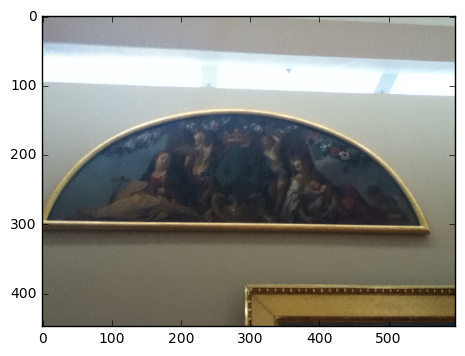
\includegraphics[width=\textwidth]{img/sample1_10A-0519.png}
\caption{Image with label 10A\label{fig:sample1_id}}
\end{subfigure}
\begin{subfigure}[b]{0.3\textwidth}
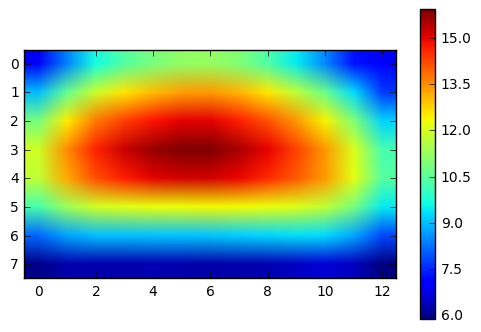
\includegraphics[width=\textwidth]{img/sample1_heatmap.png}
\caption{Heat-map for 10A\label{fig:sample1_hm}}
\end{subfigure}
\begin{subfigure}[b]{0.3\textwidth}
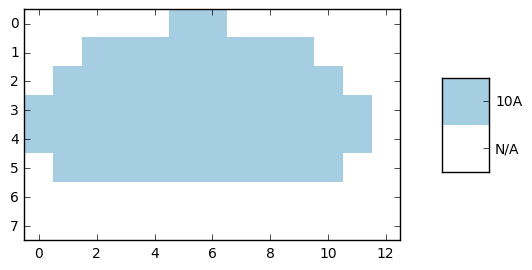
\includegraphics[width=\textwidth]{img/sample1_labels.png}
\caption{Label-map for 10A\label{fig:sample1_lab}}
\end{subfigure}

\begin{subfigure}[b]{0.3\textwidth}
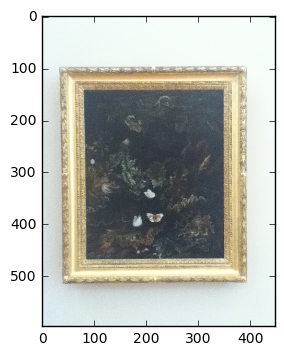
\includegraphics[width=\textwidth]{img/sample2_5P-0508.png}
\caption{Image with label 5P\label{fig:sample2_id}}
\end{subfigure}
\begin{subfigure}[b]{0.3\textwidth}
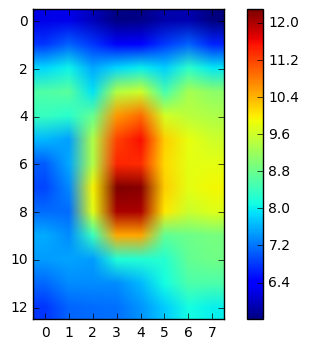
\includegraphics[width=\textwidth]{img/sample2_heatmap.png}
\caption{Heat-map for 5P\label{fig:sample2_hm}}
\end{subfigure}
\begin{subfigure}[b]{0.3\textwidth}
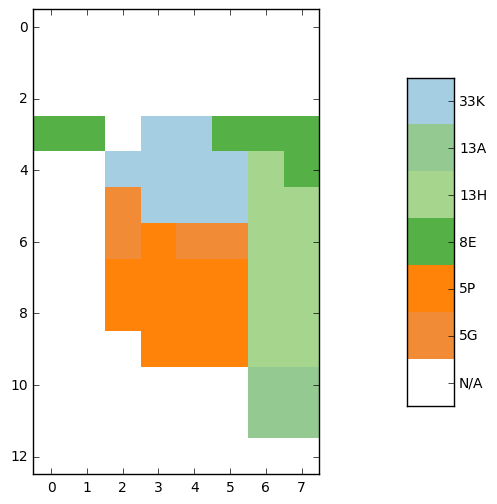
\includegraphics[width=\textwidth]{img/sample2_labels.png}
\caption{Label-map for 5P\label{fig:sample2_lab}}
\end{subfigure}

\begin{subfigure}[b]{0.3\textwidth}
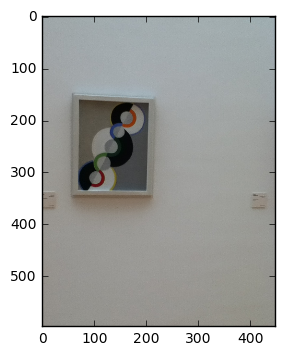
\includegraphics[width=\textwidth]{img/sample3_30P-0976.png}
\caption{Image with label 30P\label{fig:sample3_id}}
\end{subfigure}
\begin{subfigure}[b]{0.3\textwidth}
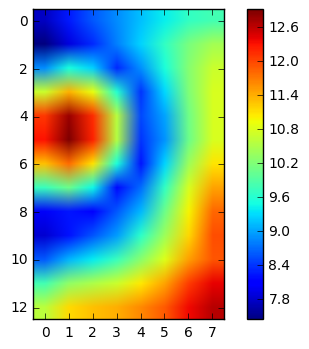
\includegraphics[width=\textwidth]{img/sample3_heatmap.png}
\caption{Heat-map for 30P\label{fig:sample3_hm}}
\end{subfigure}
\begin{subfigure}[b]{0.3\textwidth}
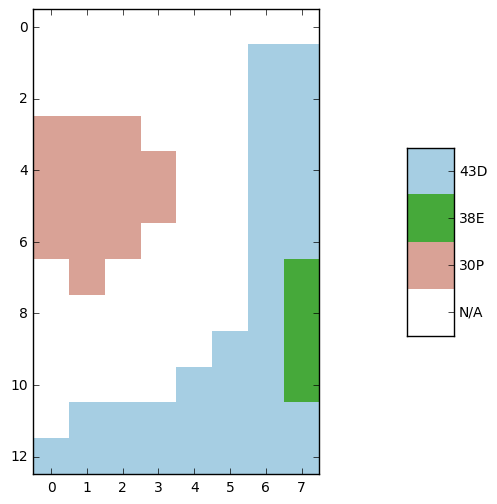
\includegraphics[width=\textwidth]{img/sample3_labels.png}
\caption{Label-map for 30P\label{fig:sample3_lab}}
\end{subfigure}
\caption{Sample images (scaled to a smaller side of 448 pixels)
along with the heat-map of maximal activation values
at each location when a fine-tuned ResNet-152 is applied to the image in a
strided manner, as well as the labels of all maximal activations that are
greater than the mean maximal activation\label{fig:heatmaps}}
\end{figure}

Figure~\ref{fig:heatmaps} shows images, along with the heat map
representing the maximal activation of a fine-tuned ResNet-152 at
each coordinate, when the network is applied in a strided manner
across the input image. The fine-tuning was carried out as described in
Section~\ref{sec:finetuning}.
From this image, we can see that the highest maximal
activations of the network usually occur at the location of the object.
This is true even if the object is not correctly classified by some of
the highest activations as can be seen in images
~\ref{fig:sample2_id}~-~\ref{fig:sample2_lab}.

In the images
~\ref{fig:sample3_id}~-~\ref{fig:sample3_lab}, it seems like many
high maximal activations occur specifically in the background area.
However, the corresponding label-map shows that these areas correspond
to the labels 38E and 43D. Both of these labels are pieces of art which
consist mostly of the background wall. In this sense, it is not
entirely wrong to consider 'wall-only' patches of the image as instances of
these pieces of art. This simply means that the image consists of two
separate regions of interest: one region with the painting (label 30P)
and one region with the wall (labels 38E/43D).

From these observations, we can confirm the assumption that the
maximal activations of a fine-tuned network are a good indicator of
the location of an object, or a combination of different objects.
Using this assumption, there is no need
for a procedure to annotate regions of interest, as employed by most
image retrieval approaches. % TODO

On the other hand, using datasets developed for image retrieval,
such as Paris6k~\cite{philbin_lost_2008} or
Oxford5k~\cite{philbin_object_2007},
this assumption cannot be applied, since the dataset is not clean
enough for a fine-tuned network to be a good indicator of location of
the query objects.

\subsubsection{Incorrectly identified images}
\begin{figure}
\centering
\begin{subfigure}{\textwidth}
\begin{tabular}{|c|*{6}{c}}
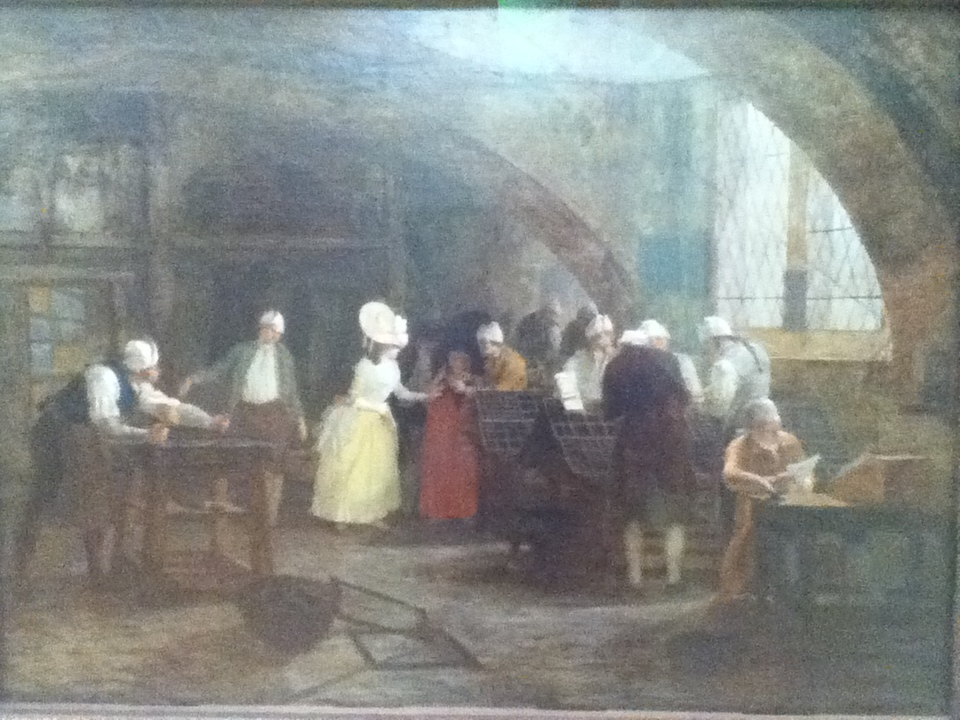
\includegraphics[width=0.12\textwidth]{img/11J-0521.JPG} &
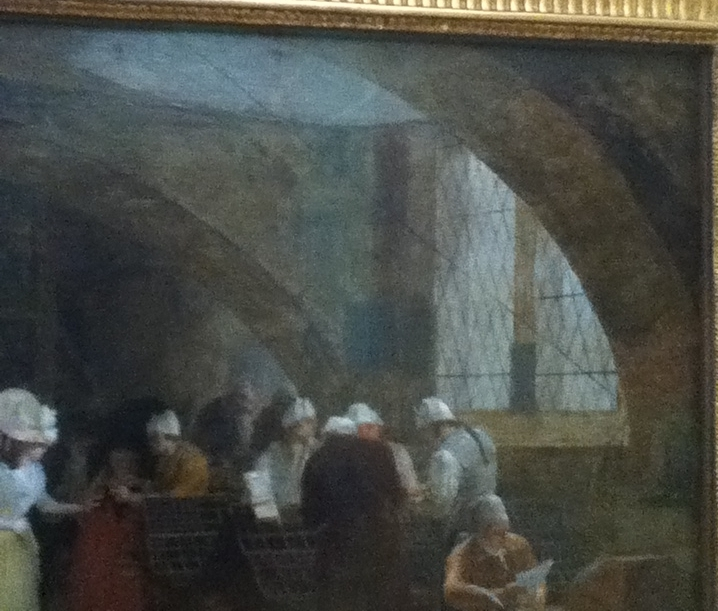
\includegraphics[width=0.12\textwidth]{img/11J-0.JPG} &
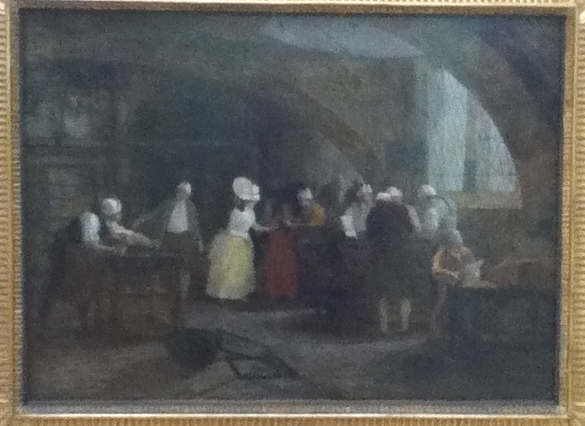
\includegraphics[width=0.12\textwidth]{img/11J-1.JPG} &
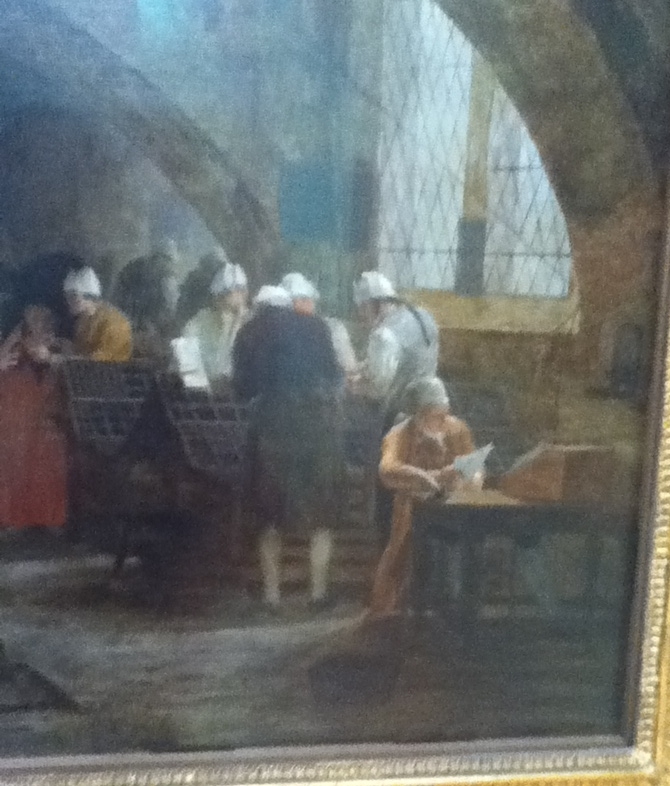
\includegraphics[width=0.12\textwidth]{img/11J-2.JPG} &
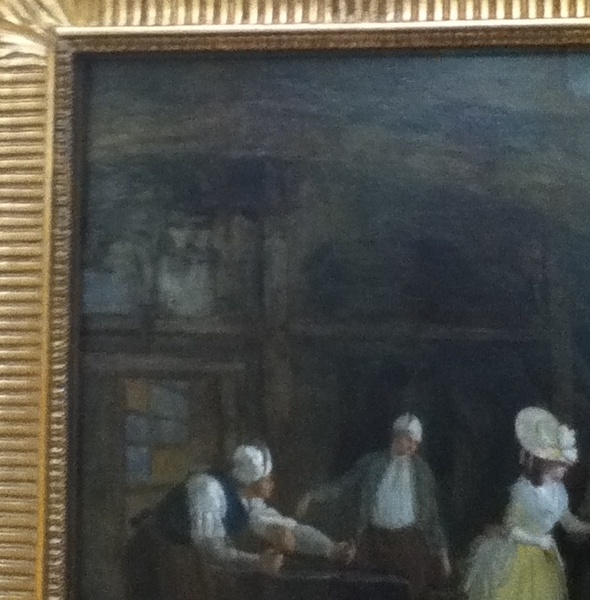
\includegraphics[width=0.12\textwidth]{img/11J-3.JPG} &
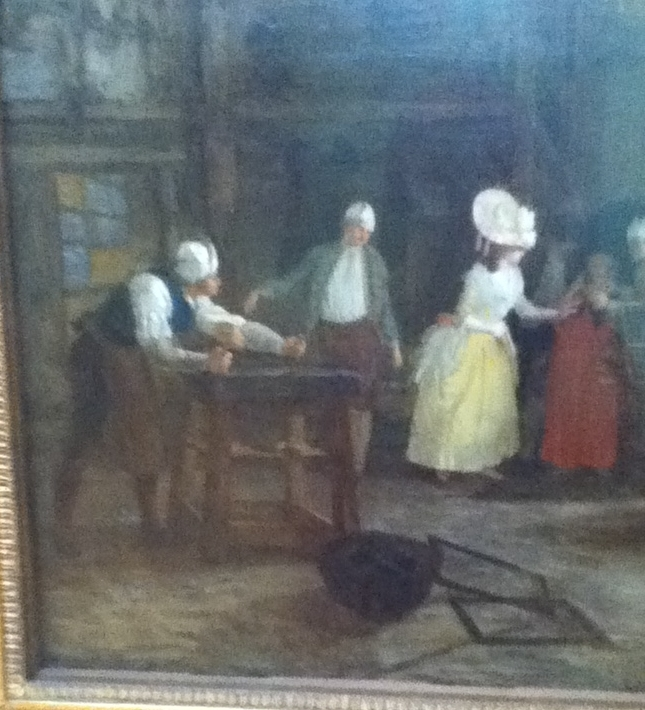
\includegraphics[width=0.12\textwidth]{img/11J-4.JPG} \\
\end{tabular}
\caption{Correctly identified query with label 11J,
along with its reference images.\newline
Average precision Gordo's net: 1.0, fine-tuned ResNet-152: 1.0
\label{fig:correct11J}}
\end{subfigure}

\begin{subfigure}{\textwidth}
\begin{tabular}{|c|*{6}{c}}
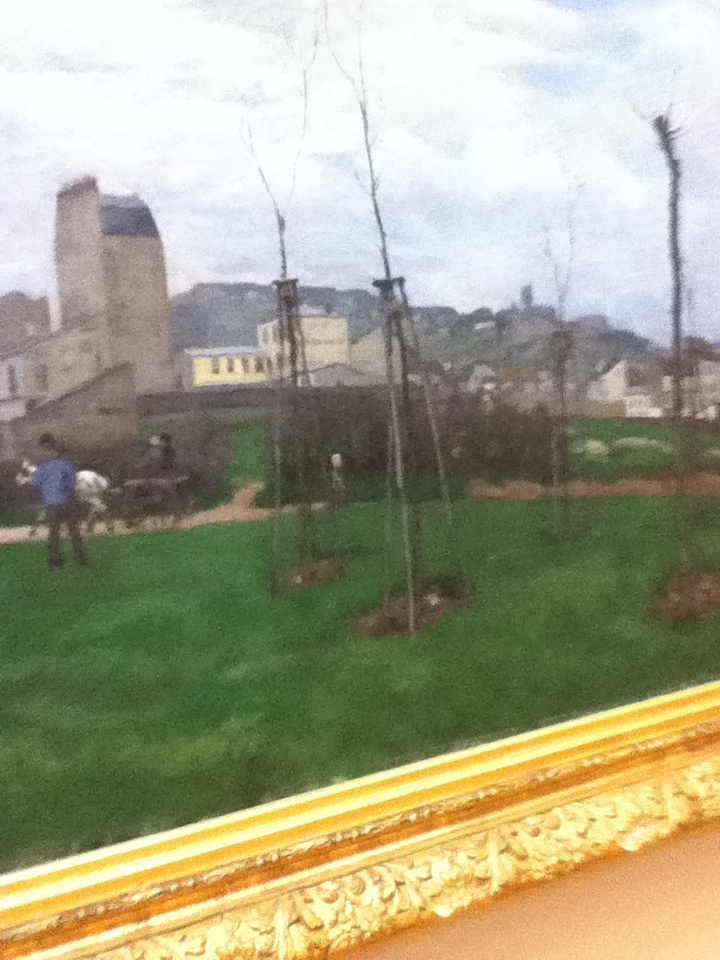
\includegraphics[width=0.12\textwidth]{img/23D-0740.JPG} &
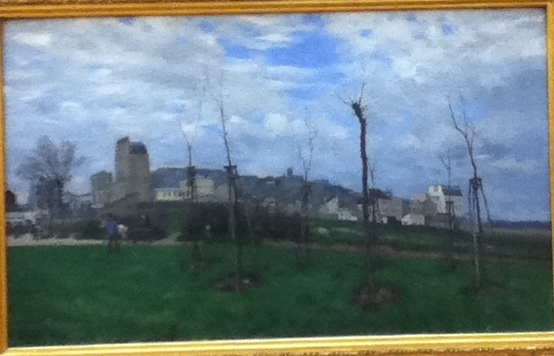
\includegraphics[width=0.12\textwidth]{img/23D-0.JPG} &
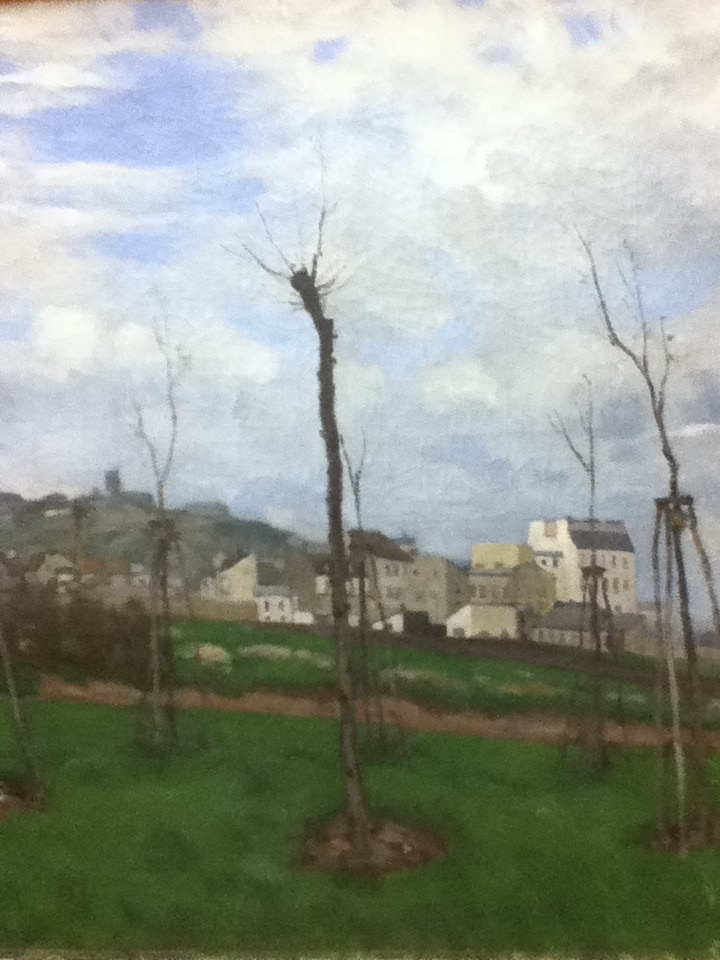
\includegraphics[width=0.12\textwidth]{img/23D-1.JPG} &
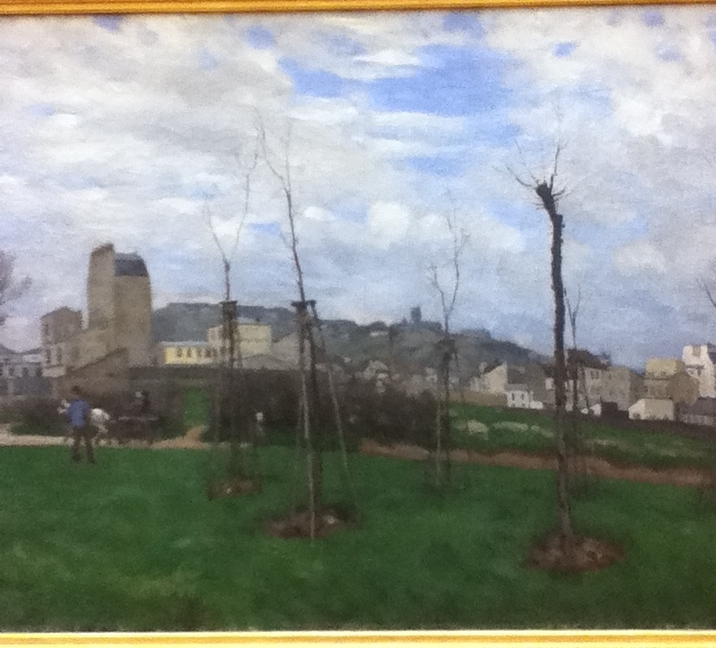
\includegraphics[width=0.12\textwidth]{img/23D-2.JPG} &
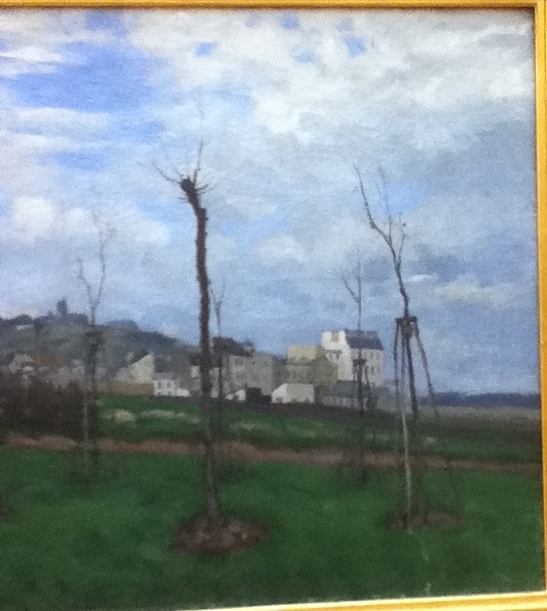
\includegraphics[width=0.12\textwidth]{img/23D-3.JPG} &
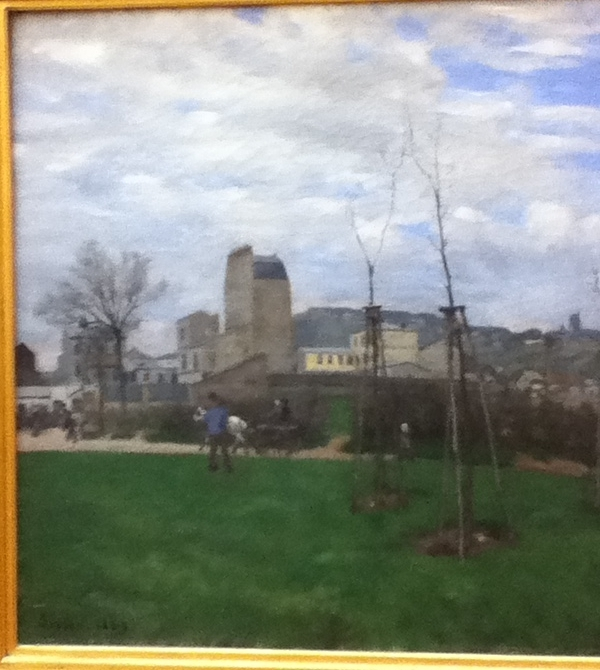
\includegraphics[width=0.12\textwidth]{img/23D-4.JPG} &
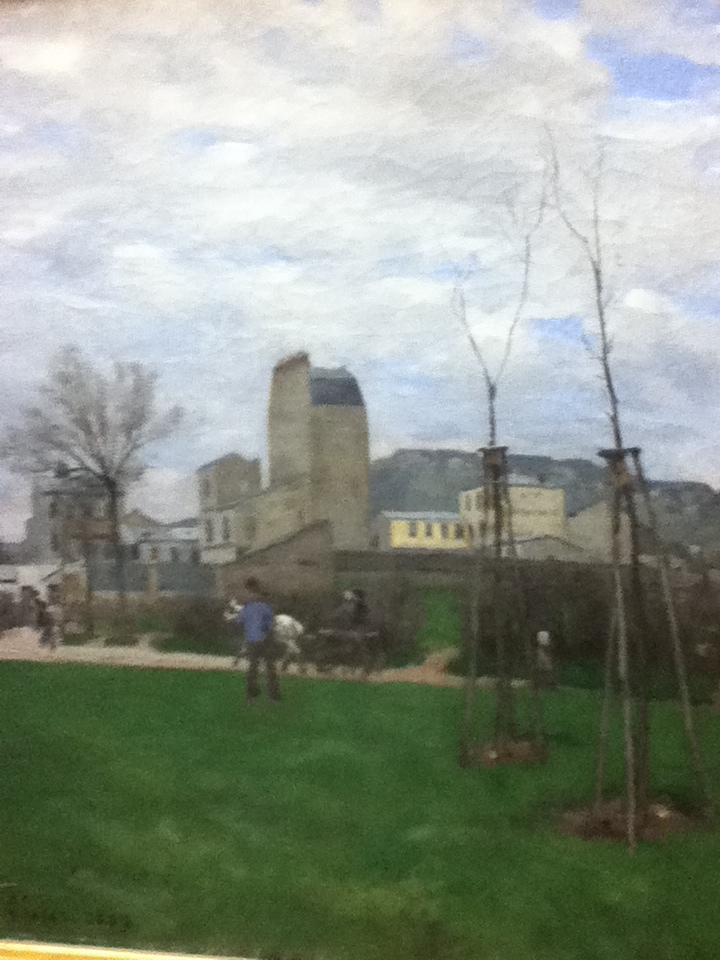
\includegraphics[width=0.12\textwidth]{img/23D-5.JPG} \\
\end{tabular}
\caption{Correctly identified query with label 23D,
along with its reference images.\newline
Average precision Gordo's net: 1.0, fine-tuned ResNet-152: 1.0
\label{fig:correct23D}}
\end{subfigure}

\begin{subfigure}{\textwidth}
\begin{tabular}{|c|*{6}{c}}
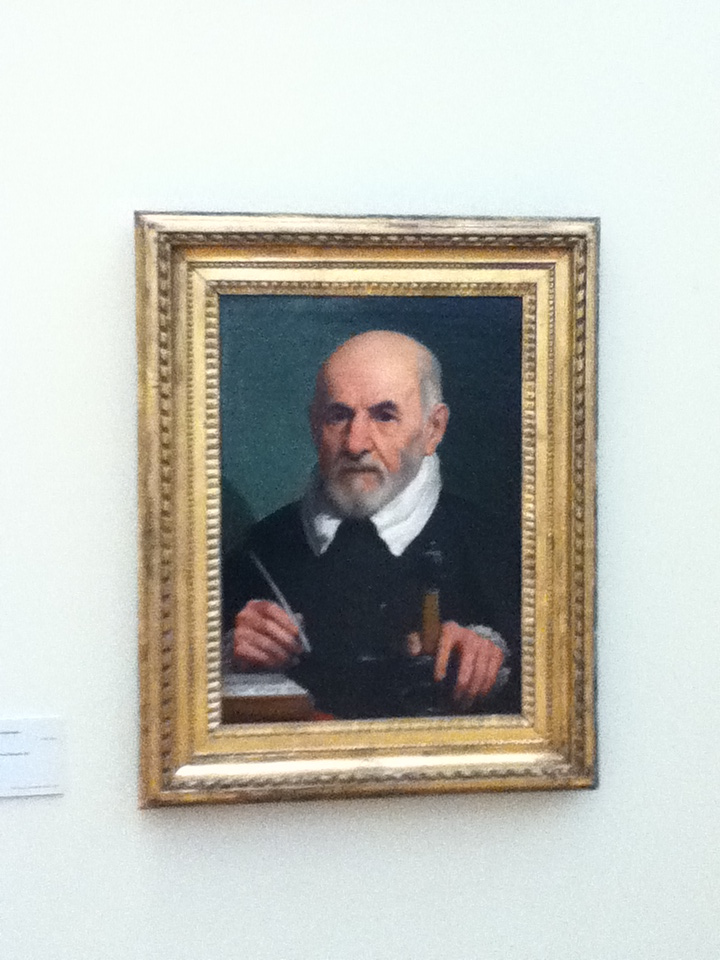
\includegraphics[width=0.12\textwidth]{img/1C-0454.JPG} &
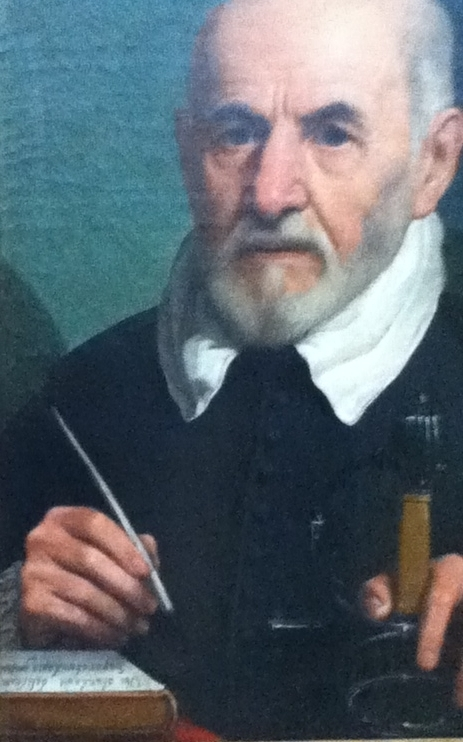
\includegraphics[width=0.12\textwidth]{img/1C-0.JPG} &
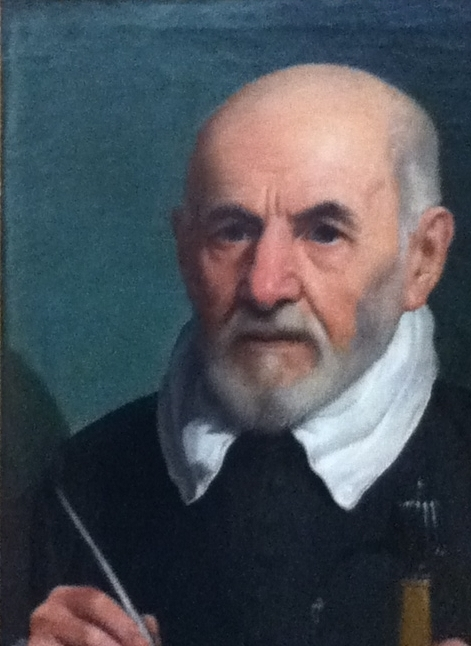
\includegraphics[width=0.12\textwidth]{img/1C-1.JPG} &
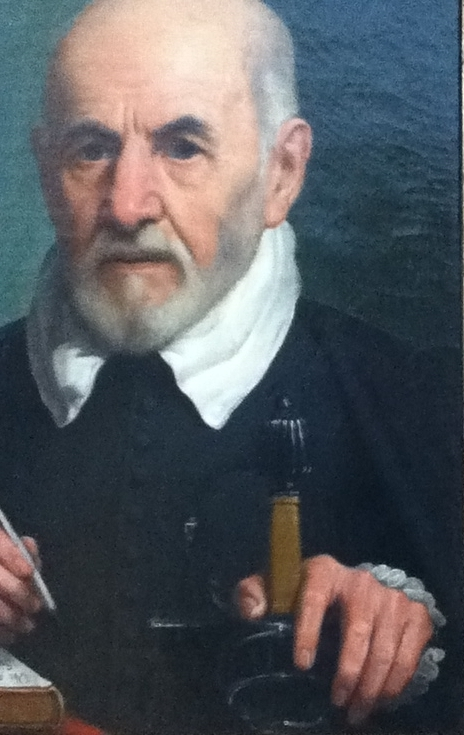
\includegraphics[width=0.12\textwidth]{img/1C-2.JPG} &
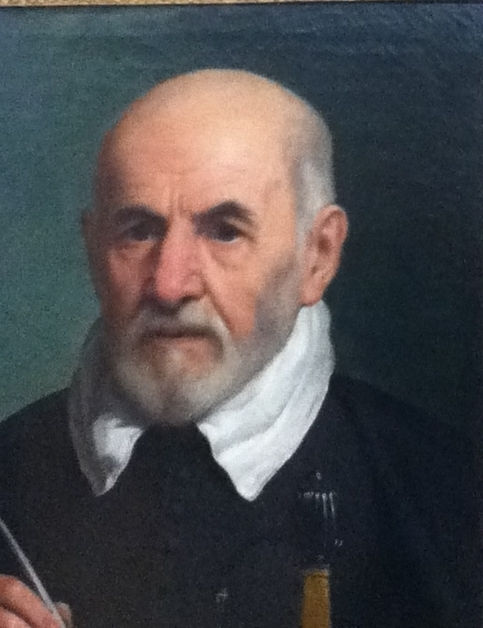
\includegraphics[width=0.12\textwidth]{img/1C-3.JPG} &
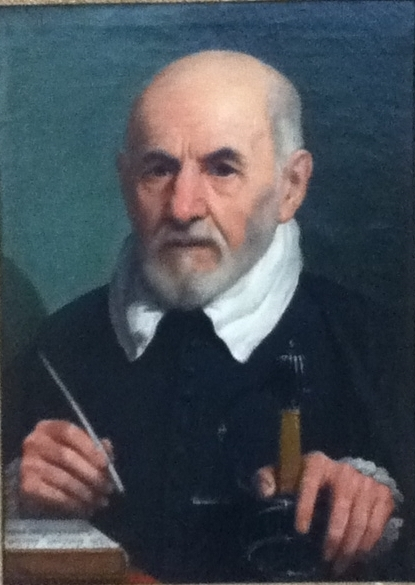
\includegraphics[width=0.12\textwidth]{img/1C-4.JPG} \\
\end{tabular}
\caption{Incorrectly identified query with label 1C,
along with its reference images.\newline
Average precision Gordo's net: 0.113, fine-tuned ResNet-152: 0.014
\label{fig:incorrect1C}}
\end{subfigure}

\begin{subfigure}{\textwidth}
\begin{tabular}{|c|*{6}{c}}
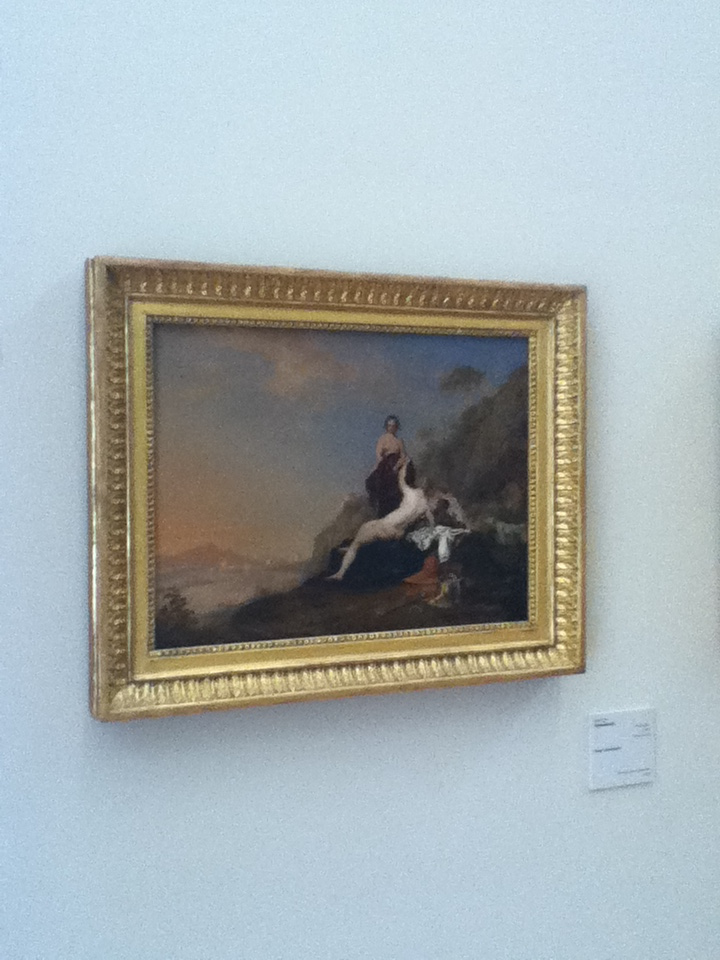
\includegraphics[width=0.12\textwidth]{img/5B-0506.JPG} &
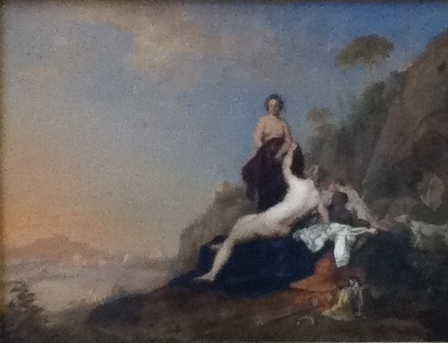
\includegraphics[width=0.12\textwidth]{img/5B-0.JPG} &
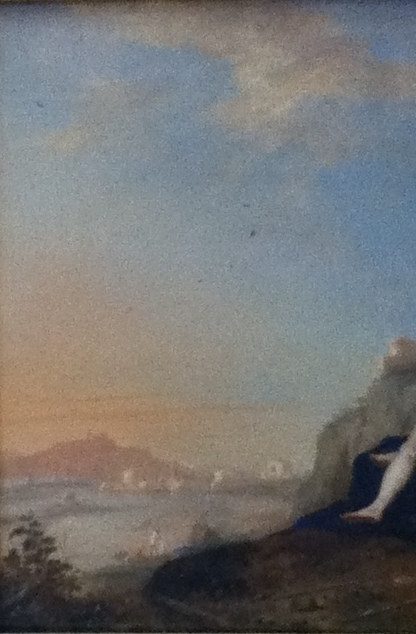
\includegraphics[width=0.12\textwidth]{img/5B-1.JPG} &
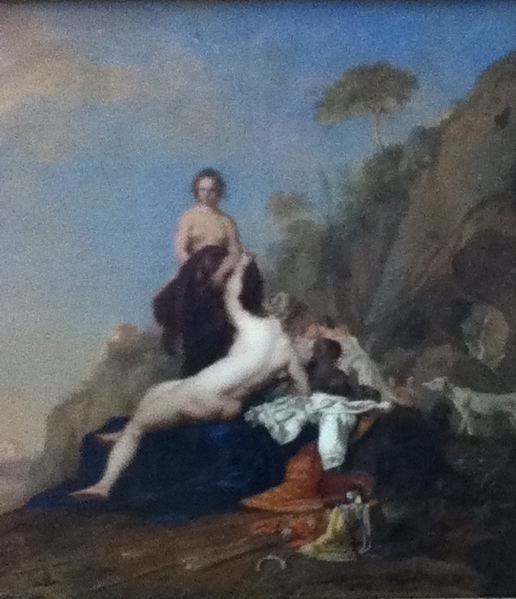
\includegraphics[width=0.12\textwidth]{img/5B-2.JPG} &
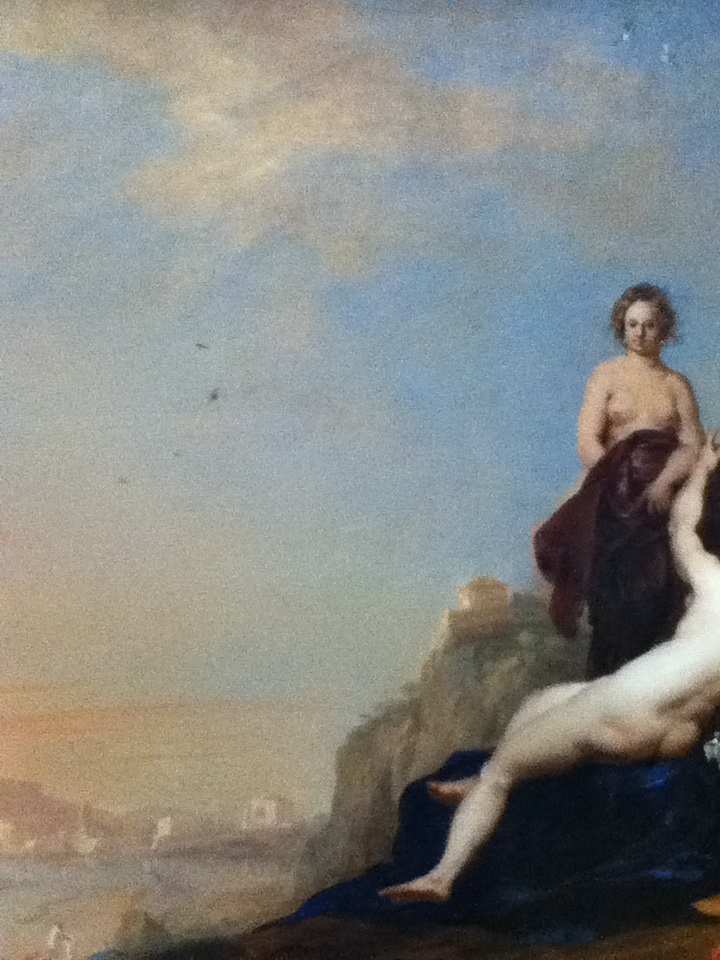
\includegraphics[width=0.12\textwidth]{img/5B-3.JPG} &
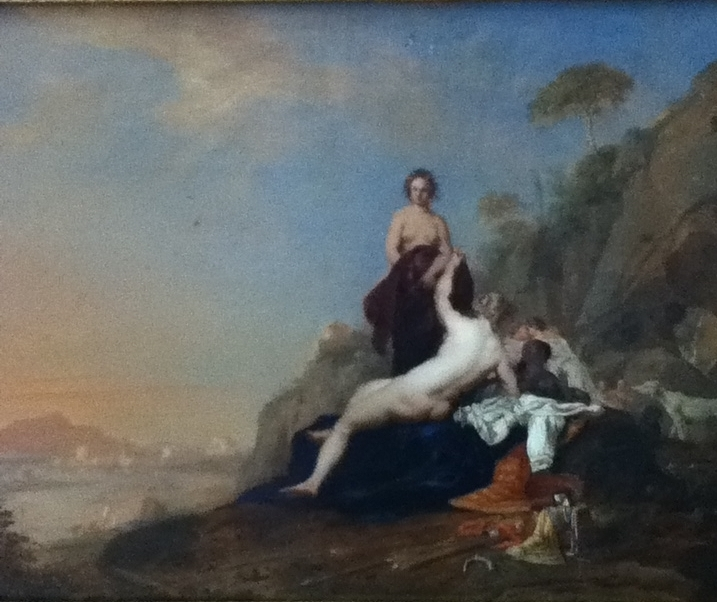
\includegraphics[width=0.12\textwidth]{img/5B-4.JPG} \\
\end{tabular}
\caption{Incorrectly identified query with label 5B,
along with its reference images.\newline
Average precision Gordo's net: 0.013, fine-tuned ResNet-152: 0.002
\label{fig:incorrect5B}}
\end{subfigure}

\begin{subfigure}{\textwidth}
\begin{tabular}{|c|*{6}{c}}
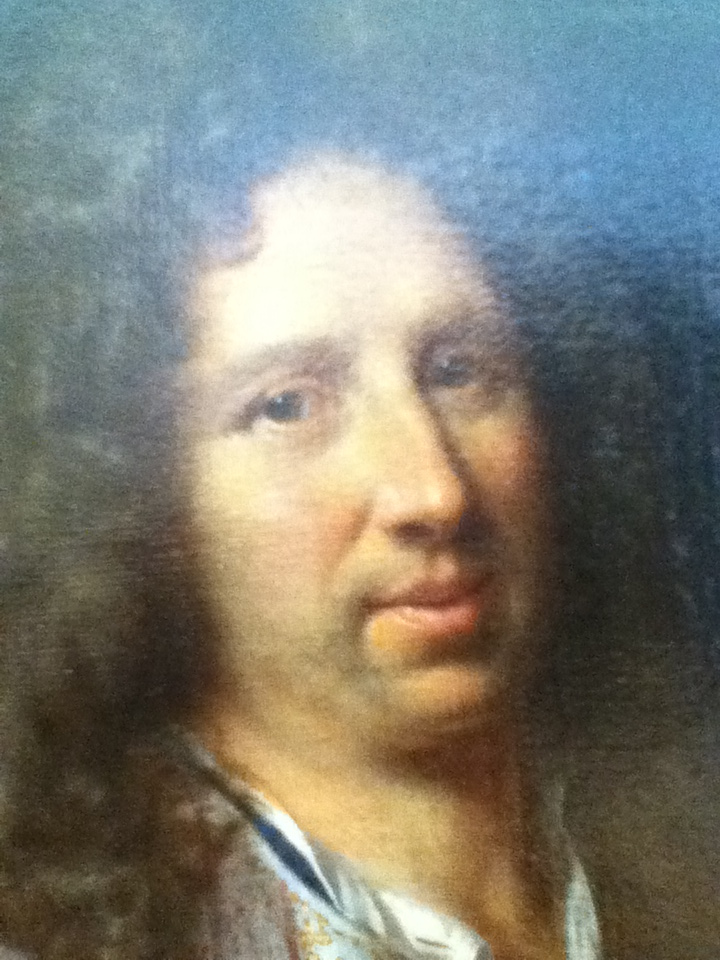
\includegraphics[width=0.12\textwidth]{img/11C-0351.JPG} &
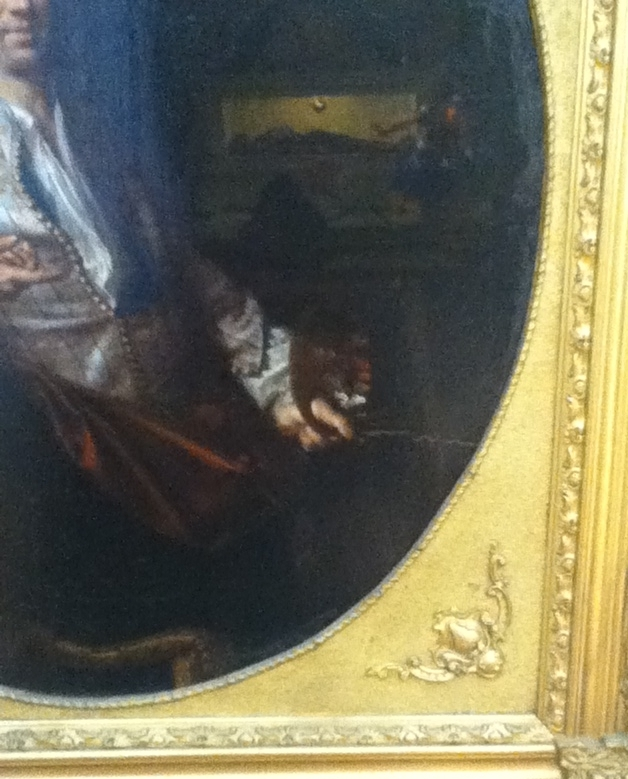
\includegraphics[width=0.12\textwidth]{img/11C-0.JPG} &
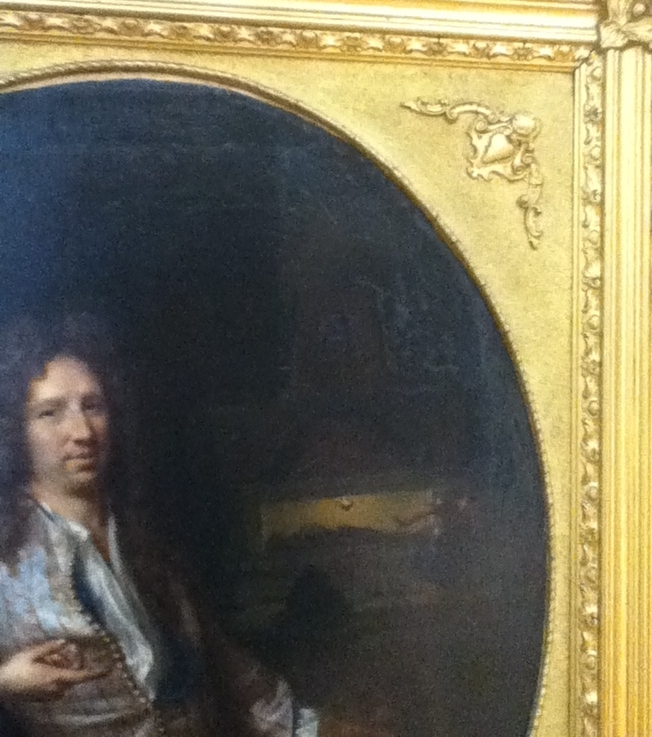
\includegraphics[width=0.12\textwidth]{img/11C-1.JPG} &
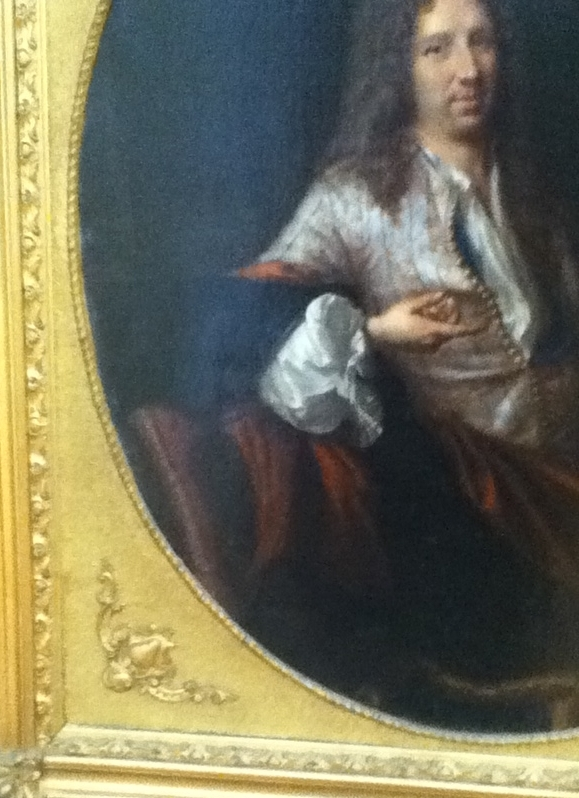
\includegraphics[width=0.12\textwidth]{img/11C-2.JPG} &
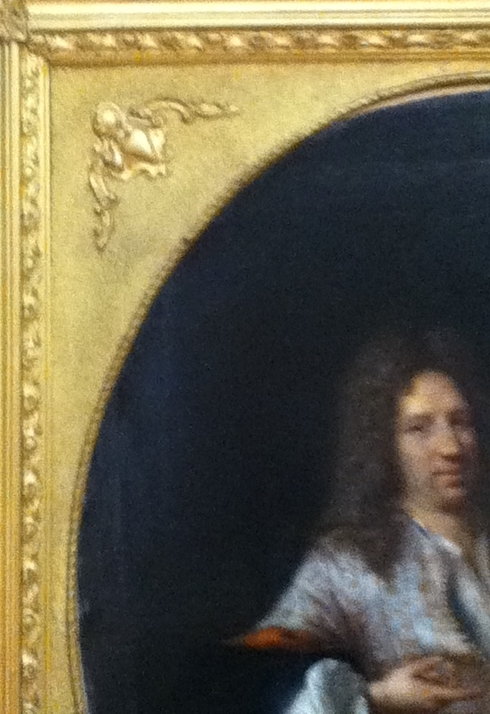
\includegraphics[width=0.12\textwidth]{img/11C-3.JPG} &
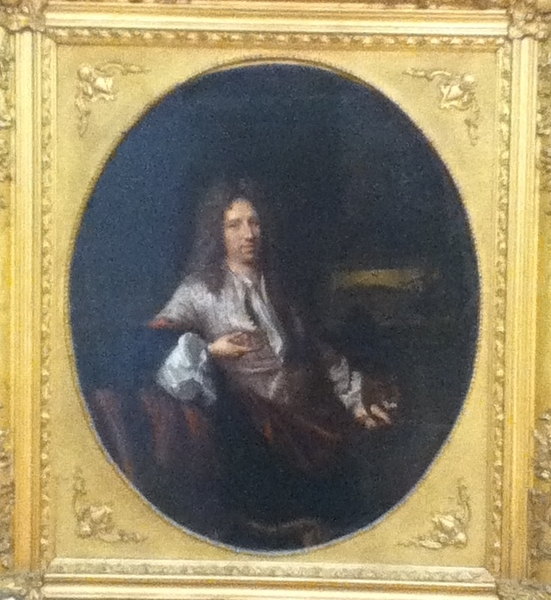
\includegraphics[width=0.12\textwidth]{img/11C-4.JPG} \\
\end{tabular}
\caption{Incorrectly identified query with label 11C,
along with its reference images.\newline
Average precision Gordo's net: 0.004, fine-tuned ResNet-152: 0.004
\label{fig:incorrect11C}}
\end{subfigure}
\caption{Sample images that were correctly and incorrectly identified
by a fine-tuned ResNet-152, as well as the network published by Gordo
et al~\cite{gordo_deep_2016}, referred to as Gordo's net. For each image,
the query image is shown at the very left and all possible correct reference
images are shown to the right of the query. The caption contains the
associated average precision values.
\label{fig:incorrectimg}}
\end{figure}

Figure~\ref{fig:incorrectimg}
shows typical images that were correctly identified versus images that
were incorrectly identified, by a fine-tuned network as well as the network
published by Gordo et al~\cite{gordo_deep_2016}, along with the average
precision for the respective queries.

From these results, we see that the networks struggle with images at
very different scales, achieving very low average precision,
while images with similar scales are usually perfectly matched.
% TODO more detail
Combining both of the properties identified in this section, we
propose a novel approach to learn a strong descriptor for instance
search in the next section.

\section{Proposed approach}
The proposed approach is based on multiple steps as described in the
following sections.

\subsection{Fine-tuning on classification using an FCN}\label{sec:fcnfinetune}
As shown in Section~\ref{sec:analysisprev}, a fine-tuned CNN is already
a good indicator of the location of an object in our datasets.
Additionally, it seems like scale is a particularly important factor.

Thus, the idea is to start by fine-tuning a network with images
at different scales. This can be achieved by using a fully
convolutional network (FCN), as introduced by
Long et al~\cite{long_fully_2015}.

In a FCN, the final fully connected layers
of a network are replaced by convolutional layers having a kernel
which fits the entire domain of the output of the previous layer.
This type of convolution is equivalent to a fully connected layer,
but allows inputs (and outputs) of any size.
The effect is that the network can be applied in one pass to an
arbitrarily sized image. The output then represents the activations
of the network as if it was applied in a strided manner across the image.
The stride of a full network depends on the architecture and is 32
pixels for the architectures used here: AlexNet and ResNet.

Once a FCN is applied to the image, the loss
is calculated by averaging the cross-entropy loss across all locations
and outputs.
The final loss is then obtained by passing images at different scales
through the FCN and averaging across all cross-entropy losses of all
outputs and scales.

When training, all images are normalized at scale to have the same
number of pixels in the smaller side. Note that for large aspect
ratios and large scales of the smaller side,
the memory consumption of training can be high for single images
having a very large aspect ratio. To limit this spike in memory
consumption, the aspect ratios are limited by introducing uniform
random noise on the smaller side of images with high aspect ratios.

\subsection{Descriptor extraction network}
\begin{figure}
\begin{subfigure}{\textwidth}
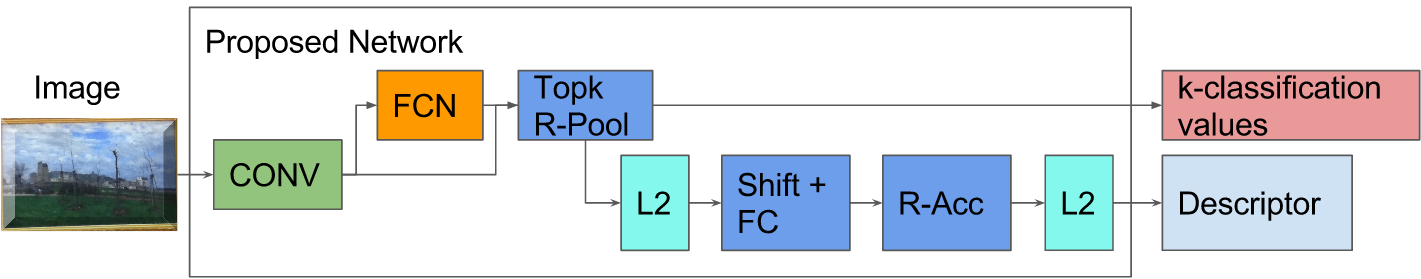
\includegraphics[width=\textwidth]{img/contrib_deploy.png}
\caption{Proposed architecture for instance search, at deploy time
\label{fig:contribdeploy}}
\end{subfigure}

\begin{subfigure}{\textwidth}
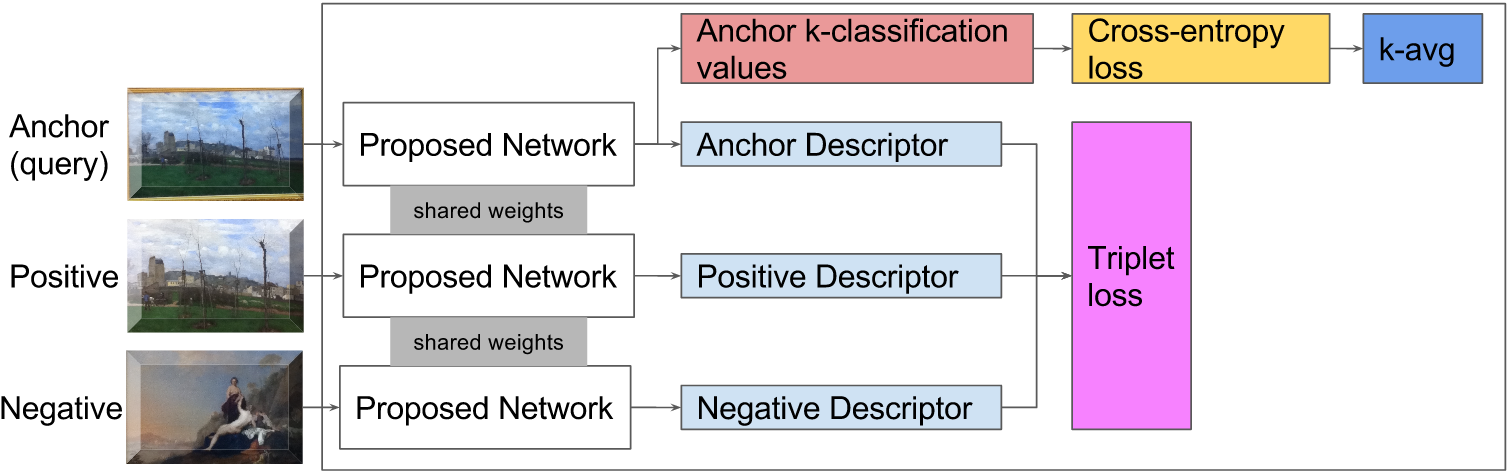
\includegraphics[width=\textwidth]{img/contrib_train.png}
\caption{Proposed architecture for instance search, at training time
\label{fig:contribtrain}}
\end{subfigure}
\caption{Proposed architecture for instance search, based on a FCN
~\cite{long_fully_2015} for region proposals. The descriptor extraction
for each region is similar to the architecture by
Gordo et al~\cite{gordo_deep_2016}, as shown in
Figures~\ref{fig:gordo_deploy}~and~\ref{fig:gordo_train}
\label{fig:contrib}}
\end{figure}

The second step of the proposed approach relies on the FCN, trained
as described in the first step in Section~\ref{sec:fcnfinetune}.

Figure~\ref{fig:contrib} illustrates the proposed architecture.
To obtain a descriptor, we first apply the convolutional layers of
a previous architecture, such as AlexNet or ResNet. We then obtain all
classification outputs at all locations using an FCN. We only consider the
maximal activation at all locations. The locations with the
top $k$ maximal activations will form the descriptor.

For each of these locations, we closely follow the architecture
proposed by Gordo et al~\cite{gordo_deep_2016}, as shown in
Figure~\ref{fig:gordo_deploy}. The convolutional features are
reduced by a L2-normalization, then a shifting and fully connected
layer. Finally, all descriptors from the $k$ locations are
sum-aggregated and L2-normalized again.

When training, the network is applied to a triplet of images.
All three descriptors are extracted and the triplet loss is
applied. To make sure that the locations with highest
maximal locations are correctly classified, a
cross-entropy loss is applied to each of the $k$ locations
used to compute the descriptor of the anchor image.
These cross-entropy losses are averaged over the $k$
locations.

\subsection{Advantages}
As shown in Section~\ref{sec:analysisprev}, this approach
allows the network to decide which region of interest is
best suited for classification and ultimately which regions
are best suited for comparison with other images.

Another advantage is that this approach does not require
any annotation of the images with regions of interest,
which can be a long, manual or automatic process, as evident
from the cleaning process used by Gordo et al~\cite{gordo_end--end_2016}.

Finally, an important property of the descriptor is that it
heavily relies on the classification
capabilities of the network. This means the descriptor is
mostly meaningless for a different dataset and needs
to be learned for each dataset. This can be an advantage,
since the descriptor can be better suited to a particular
dataset and the learning process does not take long, as shown
in Section~\ref{sec:perfresults}. On the other hand, this means that
the descriptor cannot be applied in a typical image retrieval
task.
